In diesem Kapitel werden die Arbeitsprozesse der Evaluation und Optimierung reflektiert. Des Weiteren werden Vorschläge gegeben, um das Arbeiten mit Sprachmodellen zu verbessern.\vspace{0.2cm}

Zudem werden die größten Hindernisse und Probleme besprochen, die während der es gesamten Prozesses Evaluation auftraten. Diese beinhalten die Bereitstellung er Modelle, das Erheben der Daten zu den Proben des Benchmarks und deren Auswertung. Um in folgenden Arbeiten diese Fehler zu verhindern werden dazu Lösungsansätze und Vorschläge diskutiert.

% --- Evaluierung ----------------------------------------------------------------------------------


\section{Evaluierungsaufbau und Vorbereitung}
Um die Evaluierungen an Open-Source-Modellen durchführen zu können, mussten diese lokal bereitgestellt werden. Die Wahl viel auf das Ollama-Framework, da die Installation und Konfiguration sehr gut durch den Hersteller und verschiedene Foren unterstützt wird. Neben der vorhandenen API kann das Tool \textit{Open-WebUI} einfach in das Ollama-Frameowrk integriert werden. Dieses Tool bietet eine gute UI die von allen Clients im Browser im Netzwerk aufgerufen werden kann. Ebenfalls ein großer Vorteil sind die vielen Modelle welche für Ollama zum Download bereitstehen. Darunter sind Modelle von Mistral, Llama, Deepseek und Qwen-Coder.\vspace{0.2cm}

Eine weitere Möglichkeit ist, die Modelle lokal auszuführen ohne ein Framework einzusetzen. Hierbei können die Abfragen nur auf dem lokalen System erfolgen, wenn keine eigene API Schnittstelle erstellt wird. Des Weiteren fehlte auch eine Web-UI Lösung, sodass diese Möglichkeit nicht weiter in Betracht gezogen wurde.\vspace{0.2cm}

%---------------------------------------------------------------------------------------------------


\section{Evaluierung der großen Sprachmodelle}
Ein großes Problem stellte der Zugriff auf die Cloused-Source-Modelle dar. Durch die beschränkten Bezahlmethoden konnte ein permanenter Zugriff auf die Modelle nicht erfolgen. Aus diesem Grund wurden hauptsächlich Open-Source-Modelle lokal evaluiert und getestet.


\subsection{Lokale Ressourcen}
Eines der größten Probleme für das lokale Betreiben von großen Sprachmodellen sind die Hardwareanforderungen. Hier spielen neben der Prozessoranzahl, die Speicherplatz der Festplatte und der VRAM der Grafikkarte eine entscheidende Rolle. Während der Arbeit wurde eine SSD-Festplatte mit höherer Kapazität eingesetzt und eine Grafikkarte mit mehr VRAM.\vspace{0.2cm}

Der größere Speicher wurde notwendig während des Ladens und Speichern, der Modelle von Ollama, auf die lokale SSD. Dazu war ein RAM notwendig, der doppelt so groß sein musste, wie das Modell selbst. Um diesen RAM bereit zustellen wurde eine SWAP Partition von 100 GB auf der SSD eingerichtet. Dieser wurde auch für die Ausführung größerer Modelle benötigt.\vspace{0.2cm}

Eine weitere und signifikante Verbesserung brachte der Austausch der Grafikkarte. Hierbei wurde die vorhandene Nvidia GTX 1050 TI mit 4 GB VRAM und einer Bandbreite von 112 GB/s durch eine Nvidia RTX 3060 mit 12 GB VRAM und einer Bandbreite von 360 GB/s ersetzt. Durch den Austausch der Grafikkarte wurde die eingerichtete SWAP Partition nicht mehr benötigt.

Durch diese Anpassungen bestand die Möglichkeit größere Modelle zuladen und bereit zustellt. Des Weiteren konnte eine wesentliche Verbesserung der Antwortzeit festgestellt werden. Eine genaue Messung wurde hier nicht durchgeführt. So wurden bei dem Deekseek-Coder-V2 Modelle eine Verbesserung der Berechnungszeit für den Benchmark von etwa 24 Stunden auf circa eine Stunde beobachtet.\vspace{0.2cm}

Dennoch war die Berechnungszeit für die Generierung der Codes bei einigen Modellen, die mehr als 12 GB groß waren sehr hoch. Sodass die Wartezeit, das Auswerten der Evaluierung verzögerte.


\subsection{Auswertung des Benchmarks}
Die Anwendung des vorgeschlagenen Parametersatzes zeigte bemerkenswerte unerwünschte Auswirkungen auf die Erzeugung der Antworten. Insbesondere bei einer Tokenlänge von 600 traten Störungen auf, bei denen einige Modelle unbrauchbaren Code generierten. Dieser Umstand resultierte beim \textit{DeepSeek-R1} aus einem 'explanation'-Abschnitt innerhalb der Antwortstruktur, in dem das Modell eine detaillierte Herleitung seines Denkprozesses anbot, bevor es zur eigentlichen Lösung gelangte. Bei dem Modell \textit{Gemini 1.5} führten ausführliche Erklärungen am Anfang und am Ende der Antwort zum selben Effekt, sodass diese Ergebnisse ebenfalls nicht brauchbar waren. Aus diesem Grund wurde beim \textit{DeepSeek-R1} und beim \textit{Gemini 1.5} auf eine Einschränkung der Tokenlänge verzichtet. Auf eine erneute Evaluierung des OpenAI Modell musste aus Kostengründen verzichtet werden.\vspace{0.2cm}

Bei der Auswertung des Benchmarks traten einige Fehler auf, die beseitigt werden konnten. Ein Großteil waren kleinere Fehler, die bei der Auswertung aufgetreten, die in Kapitel \ref{subsec:disadvantages_of_evaluation} ausführlicher besprochen werden. Der gravierendste Fehler trat aber bei der Berechnung das \texttt{pass@k} für das gesamte Modell auf. Hier wurde eine falsche Python-Methode implementiert, sodass die Ergebnisse, um ein Vielfaches niedriger waren. Erst durch den Vergleich mit Ergebnisse anderer Arbeiten und den Herstellerangaben ist der Fehler aufgefallen. Nach intensiver Suche wurde dieser schlussendlich gefunden und beseitigt.\vspace{0.2cm}

Bewehrt hat sich der Einsatz von Python und dessen Bibliotheken für Umsetzung der Evaluierungs- und Optimierungsaufgaben. Mittlerweile existieren für die meisten Probleme und Anforderungen bereits fertige Bibliotheken. Oft von den Herstellern der Modelle selbst. Basierend auf den vorhandenen Bibliotheken, konnte die Entwicklung der Evaluationsaufgaben in kurzer Zeit umgesetzt und implementiert werden.\vspace{0.2cm}

% --- Evalierung mit eigenen ---------------------------------


\subsection{Nachteile der Evaluierung}\label{subsec:disadvantages_of_evaluation}
Trotz seines häufigen Einsatzes bei der Evaluierung von Modellen, in verschiedenen wissenschaftlichen Arbeiten, zeigt der Benchmark-Test für die deutschen PHP Proben Fehler. Aber auch bei der Erstellung der Auswertung mit Python traten Fehler auf. Dadurch entstehen Nachteile für die Modelle, bei der Bewertung mit dem HumanEval-XL Benchmark. Im Verlauf dieses Kapitels werden einige Nachteile diskutiert.\vspace{0.2cm}

Bei der Probe \textit{php/5} wurde eine \textit{\textbf{nicht eindeutige Übersetzung}} festgestellt. So wurde die Probe übersetzt, nicht aber die Tests. Das Listing \ref{lst:prompt_php_de_5} zeigt die gültigen Werte welche als Eingabeparameter für die zu generierende Funktion erlaubt sind. Hier handelt es sich um deutsche Zahlworte von $null$ bis $neun$. Im angegebenen Beispieltest sind Eingabe- und Ausgabeparameter in englischer Sprache. Es wird auch nicht explizit angegeben, das eine Übersetzung erfolgen soll.\vspace{0.2cm}

\begin{lstlisting}[
language=php,
label=lst:prompt_php_de_5,
caption={Aufgabenstelleung der Probe php/5}
]
/**
 * Sie sind ein erfahrener PHP-Programmierer und hier ist Ihre Aufgabe.
 * Die Eingabe ist ein durch Leerzeichen getrennter String von Ziffern von 'null' bis 'neun'.
 *     Gültige Optionen sind 'null', 'eins', 'zwei', 'drei', 'vier', 'fünf', 'sechs', 'sieben', 'acht' und 'neun'.
 *     Gib den String mit den Zahlen sortiert von klein nach groß zurück.
 * >>> sort_numbers('three one five')
 * 'one three five'
 *
 */
function sortNumbers($numbers){
\end{lstlisting}

Der Test der Probe \textit{php/5}, welcher in Listing \ref{lst:test_php_de_5} zu sehen ist, erstellt eine Prüfung der generierten Methode mit englischem Zahlworten von $zero$ bis $nine$ bereit. Keines der getesteten Modelle hat diese Probe bestanden.

\begin{lstlisting}[
	language=php,
	label=lst:test_php_de_5,
	caption={Aufgabenstelleung der Probe php/5}
]
// more tests.

$arg40 = "six five four three two one zero";
$x4 = sortNumbers($arg40);
$v4 = "zero one two three four five six";
if (!compare($x4, $v4)) {
    throw new Exception("Error at 5th assert statement.");
}
\end{lstlisting}

Eine mögliche Lösung ist die Anpassung des Benchmarks vorzunehmen und alle Übersetzungen anzupassen oder zu korrigieren. Mit der originalen Benchmark PHP Probendatei, hat beispielsweise das Modell \textit{Deepseek Coder V2} dasselbe beschriebene Problem und kann keine, nach dem Test im Benchmark korrekte Lösung generieren. Wird der Test im Benchmark angepasst und die Zahlworte ebenfalls übersetzt, so wie der in Listing \ref{lst:test_php_de_5_translated} gezeigte Teil, wird die Probe von dem Modell mit drei korrekten Antworten bestanden. Derselbe Test in der englischen Sprache wurde vom Modell \textit{Llama3.3} in allen fünf Antworten, mit bestanden bewertet.\vspace{0.2cm}

\begin{lstlisting}[
	language=php,
	label=lst:test_php_de_5_translated,
	caption={Übersetzte Aufgabenstelleung der Probe php/5}
]
// more tests.

$arg40 = "sechs fünf vier drei zwei eins null";
$x4 = sortNumbers($arg40);
$v4 = "null eins zwei drei vier fünf sechs";
if (!compare($x4, $v4)) {
    throw new Exception("Error at 5th assert statement.");
}
\end{lstlisting}

Die Ergebnisse für die fünfte Probe vor und nach der Änderung sind im Listing \ref{lst:test_php_de_5_translated_bash_view} dargestellt. Nach dem Namen $php/5$ wird die Gesamtanzahl der Proben angegeben, gefolgt von den insgesamt bestandenen Durchläufe der Probe. Anschließend werden die Wahrscheinlichkeiten, das eine korrekte Antwort unter den TOP Antworten zu finden ist, angegeben, beginnend mit dem \texttt{pass@1}.\vspace{0.2cm}

\begin{lstlisting}[
	language=bash,
	label=lst:test_php_de_5_translated_bash_view,
	caption={Ergebnisse der Probe php/5 für das \textit{Deepssek Coder V2} Modell}
]
# origin sample no. 5
php/5;5;0;0.0000;0.0000;0.0000;0.0000;0.0000

# translated sample no. 5
php/5;5;3;0.6000;0.9000;1.0000;1.0000;1.0000
\end{lstlisting}

Diese Probe zeigt, nach der Änderung wurden drei von fünf möglichen Antworten mit korrekt bewertet. Die Änderung für die Bewertung der \texttt{pass@k} Methode des gesamten Modells ist in Tabelle \ref{tab:pass_at_k_results_bevor_after_translate} dargestellt. Diese Änderung wurde nicht mehr auf alle Modelle ausgeweitet, sodass der Fehler in allen Bewertungen enthalten ist.\vspace{0.2cm}

\begin{table}
	\begin{tabular}{|l|lllll|}
		\hline
		k & 1 & 2 & 3 & 4 & 5 \\
		\hline
		ohne Korrektur & 0,555 & 0,6112 & 0,6312 & 0,6425 & 0,65 \\
		mit Korrektor  & 0,565 & 0,6225 & 0,6438 & 0,6550 & 0,6625 \\
		\hline
		\hline
	\end{tabular}\centering
	\label{tab:pass_at_k_results_bevor_after_translate}
	\caption{Ergebnisse für das \textit{Deepseek Coder V2} Modell mit und ohne Probe 5 Korrektur }
\end{table}

Mit diesem Problem wird gezeigt, dass bereits ein kleiner Fehler das Ergebnis um mehr als ein Prozent für ein Modell verbessern kann.\vspace{0.2cm}

Eine andere Fehlerquelle ist das \textit{\textbf{Zusammenführen der Antworten der Modelle und Tests aus dem Benchmark}}. Diese Fehlerquelle ist nicht der Benchmark selbst, sondern die Umsetzung der Ausführung und Bewertung. Oft sind die Probleme das Parsen der Sonderzeichen, wie beispielsweise die Verwendung der doppelten Anführungszeichen im Test und den erstellten Antworten. Eine manuelle Prüfung der Aufgabe 2 hat das Fehlverhalten aufgezeigt. Durch das Implementieren einiger weiteren Codezeilen in Python, wie das Listing \ref{lst:error_evaluation_code_1} zeigt, konnten die Bewertung einiger Modelle verbessert werden. So hat sich die Bewertung für die \textit{pass@1} Methode des Deepseek-Coder-V2 um 7\% von $0,53$ auf $0,6$ verbessert. Ebenso wurde für das Llama3.1 Modell eine Verbesserung der Bewertung um $0,025$, von $0,45$ auf $0,475$ ermittelt.\vspace{0.2cm}

\begin{lstlisting}[
	language=diff,
	label=lst:error_evaluation_code_1,
	caption={Fehler bei der Auswertung durch fehlerhafte Anführungszeichen}
]
answer = answer.replace(r"\n", "\n")
+ answer = answer.replace(r'\"', '"')
+ 
+ test = test.replace(r'\"', '"') 
\end{lstlisting}

Ein weiteres Problem, welches sich in den Tests gezeigt hat, sind die von einigen Modellen \textit{\textbf{verwendeten umgeänderten Methodennamen}}. Einige Modelle ändern diesen ab und passen ihn an die Funktionalität der Methode an. Dieses Verhalten ist beispielsweise beim Google Modell \textit{Gemini 1.5} mehrfach aufgetreten. Ein Beispiel ist die Probe 26 aus dem Benchmark. Hierbei sollte das $n$-te Element der Fibonacci-Folge berechnet werden. Der geforderte Name der Methode war als \texttt{fibfib} definiert. Das Modell schlug in einem Durchlauf den Namen \texttt{fibfib\_iterativ} vor, da über ein beliebig großes $n$ iteriert wird. Somit ist der Test für diese Probe fehlgeschlagen, obwohl die Methode die Berechnung korrekt durchführte. Das Listing \ref{lst:correct_func_with_non_correct_name} zeigt diese, durch \textit{Gemini 1.5} generierte Funktion.\vspace{0.2cm}

\begin{lstlisting}[
	language=php,
	label=lst:correct_func_with_non_correct_name,
	caption={Generierte Funktion mit falschen Namen}
]
function fibfib_iterativ($n) {
    if ($n < 0) {
        throw new InvalidArgumentException("n muss nicht-negativ sein");
    }

    if ($n <= 2) {
        return $n - 1;
    }

    $a = 0;
    $b = 0;
    $c = 1;
    for ($i = 3; $i <= $n; $i++) {
        $temp = $a + $b + $c;
        $a = $b;
        $b = $c;
        $c = $temp;
    }
    return $c;
}
\end{lstlisting}

Ein menschlicher Entwickler würde den Methodennamen anpassen und die Methode einsetzen. Eine Möglichkeit dies zu umgehen, ist es, den Methodennamen zur Laufzeit zu ermitteln. Mit den Proben sollen die Fähigkeiten der LLMs geprüft werden, inwieweit diese, grundlegende Funktionen implementieren können. Hierbei ist der Name der Methode nicht entscheidend. Anders verhält es sich bei Erweiterungen bestehender Programme, bei denen die erstellten Funktionen integriert werden sollen.\vspace{0.2cm}

Die Tests aus dem Benchmark und Ergebnisse der Modelle wurde stichprobenartig manuell geprüft und weitere Fehler behoben. Dennoch ist nicht auszuschließen das die jetzige Evaluation weitere Fehlerquellen enthält.\vspace{0.2cm}

Es gibt durchaus weitere Fehlerquellen, welche die Ergebnisse negativ beeinflussen können. Bei der Formulierung der Tests könnten Randbedingungen nicht korrekt betrachtet wurden sein, was dazu führen kann, dass der Einsagt der generierten Codes zu Fehlern führen könnte. Ebenfalls können die Tests falsche Parameter vorgeben, wodurch korrekt generierter Code als falsch bewertet wird. Die eben genannten Fehler konnten im vorliegenden Ergebnissen nicht nachgewiesen werden, ganz auszuschließen sind sie aber nicht.\vspace{0.2cm}

% --- Optimierung ----------------------------------------------------------------------------------


\section{Optimierung der Abfragen}
Wie bereits in Kapitel \ref{sec:conzept_of_optimization_prompt} besprochen sind die Prompts in den Benchmarks sehr gut optimiert. Die Optimierungstests mit der Auswahl eines anderen Framework hat zu einer erheblichen Steigerung der Ergebnisse geführt. Diese signifikante Verbesserung wurde so nicht erwartet. Dieses Ergebnis zeigt, dass die Prompts in des HumanEval-XL Benchmarks weiter optimiert werden können. Zum anderen zeigt es, dass das DSPy Framework die Prompts selbstständig optimiert, ohne das Entwickler tiefgehende Kenntnisse im Prompt Engineering haben müssen.\vspace{0.2cm}

Dennoch zeigt der Test auch, dass diese Optimierung Grenzen hat. So konnte sich beim \textit{Llama 3.1} keine Optimierung erzielt lassen. Hier sind die Ergebnisse schlechter ausgefallen. Für die Optimierungstests wurde eine Konfiguration aus dem DSPy Framework getestet. Das Framework bietet verschiedene Möglichkeiten der Datenverarbeitung, in diesem Fall das Optimieren der Prompts. Hierbei könnten weitere Konfigurationen bestehend aus Signatur und Modul getestet werden die das Framework mitbringt und zusätzlich an eigene Bedürfnisse anpassbar ist.\vspace{0.2cm}

In den Auswertungen der Optimierung sind einige Modelle nicht aufgeführt, da das \texttt{DSPy} Framework bei den Anfragen der Proben an die Modelle mit Fehlern abbricht. Hierbei handelt, ist sich um das Codelama-Modell \textit{codellama:70b-instruct-q2\_K}. Abfragen mit \texttt{langchain} Framework zeigen diese Fehler nicht. Das gleiche Verhalten ist bei weiteren größeren Modellen, wie das \textit{llama3.3:70b} und \textit{deepseek-r1:32b} zu beobachten. Es wurden verschiedene Module, darunter \texttt{Predict}, \texttt{ProgramOfThought} oder \texttt{ChainOfThought} und Signaturen getestet, zum Zeitpunkt der Arbeit wurde keine Lösung für dieses Problem gefunden.\vspace{0.2cm}

Eine mögliche Ursache, kann darin liegen, dass \texttt{DSPy} einen deklarativen Ansatz implementiert und im Gegensatz zu \texttt{langchain}, Abfrageketten erstellt. Hierbei besteht die Möglichkeit, dass unvollständige Ergebnisse, die von den LLMs gesandt werden, nicht so effektiv vom Framework verarbeitet werden, wie es bei \texttt{langchain} der Fall ist. Hierbei könnte der Fehler dadurch entstehen, da der zur Verfügung stehen VRAM des Servers auf 12 GB beschränkt ist und somit könnten größere Modelle unvollständige Antworten erstellen. Bei allen drei Modellen übersteigt die Modellgröße den verfügbaren VRAM.  Das Problem konnte nicht abschließend aufgeklärt werden.\vspace{0.2cm}

\begin{figure}[!ht]
	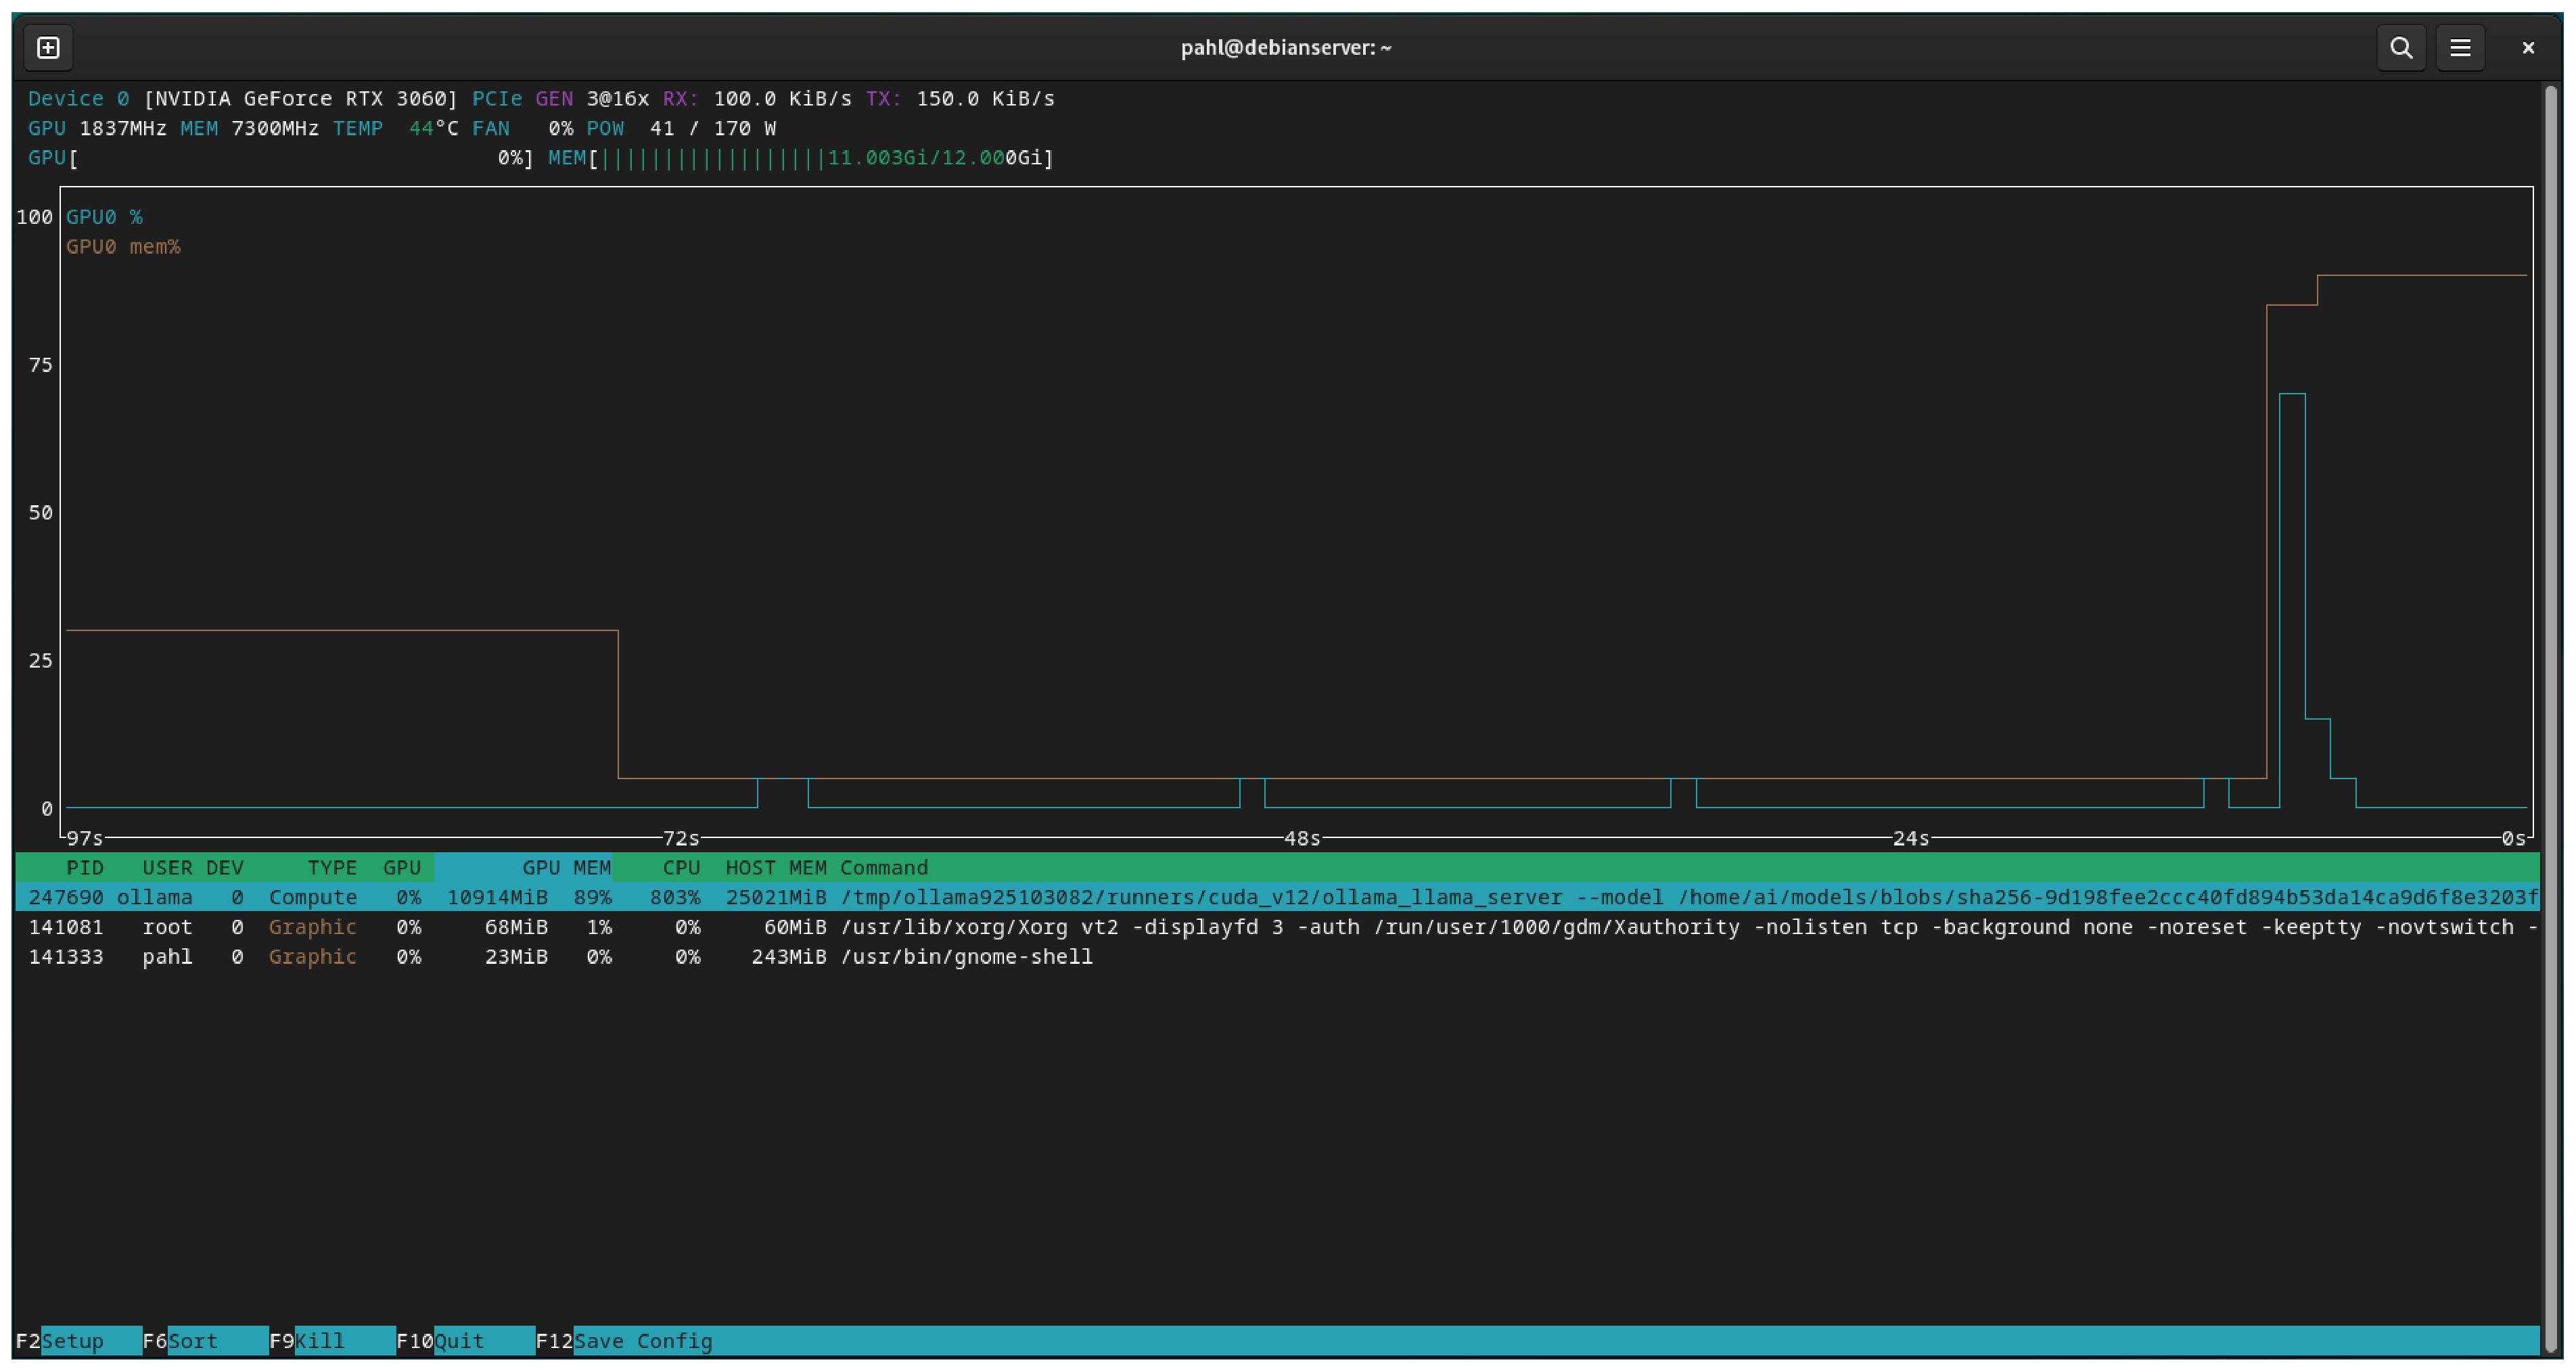
\includegraphics[width=0.8\textwidth]{content/chapter_lessons_learned/images/nvtop_model_change.eps}
	\centering
	\caption{Auslastung des VRAMs während eines Modellwechsels}
	\label{img:bash_nvtop_model_change}
\end{figure}

Die Abbildung \ref{img:bash_nvtop_model_change} zeigt den Modellwechsel vom \textit{Llama3.2} zum \textit{Codellama:70b} Modell. In der Abbildung werden die Grafikkartenparameter mit dem Tool \texttt{nvtop} ausgelesen und angezeigt. Während die Auslastung des VRAMs beim \textit{Llama3.2:3b} 3,64 GB beträgt, sind es beim \textit{Codellama:70b} mehr als 11 GB. Das \textit{Llama3.2:3b} hat eine tatsächliche Größe von 2 GB, während das \textit{Codellama:70b} eine tatsächliche Größe von 25 GB hat. Im linken Teil der Abbildung ist das geladene \textit{Llama3.2:3b} Modell zusehen, gefolgt von einem Leerlauf des Speichers zur Vorbereitung auf das neu zu ladende \textit{Codellama:70b} Modell. Die Speicherauslastung dieses Modells ist auf der rechten Seite der Abbildung \ref{img:bash_nvtop_model_change} zu erkennen.
